\subsection{Estrutura de um Clock Físico}

Fisicamente, um sinal de clock é gerado por um oscilador e, apesar de extistírem diverssas formas de implementar um oscilador, tipicamente são baseados em cristal de quartzo ou circuitos eletrônicos ressonantes equivalentes.

\begin{figure}[H]
    \centering
    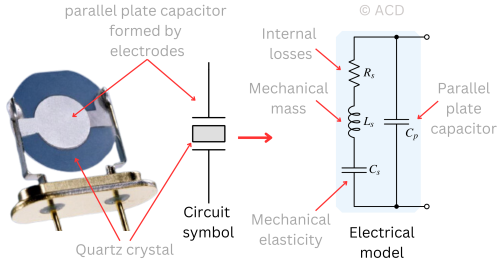
\includegraphics[width=0.7\linewidth]{images/Quartz Oscilator.png}
    \caption{Oscilador de Quartzo\cite{analog_oscillators_notes}.}
    \label{fig:Quartz Oscilator}
\end{figure}


O cristal de quartzo é um cristal Piezoelétrico, em verdade, foi o primeiro cristal dessa categoria descoberto \cite{mould_piezo}. Tais cristais, devido a sua estrutura molecular não centrocimétrica, isto é, com distribuição de cargas assimétricas, conduzem corrente quando deformados e são isolantes em estado de relaxamento \cite{mould_piezo}. Dado um potencial inicial, o cristal deforma, conduz corrente e depois oscila em sua frequencia de ressonancia natural \cite{mould_quartz}.

Entretanto, com o decorrer do tempo, a energia do sistema é dispersa e as oscilações do circuito ressonante diminuem em amplitude até que parem completamente no equilíbrio. Por isso, além do oscilador ressonante, é necessário um sistema de feedback e amplificação do sinal, para que esta oscilação seja mantida. 

\begin{figure}[H]
    \centering
    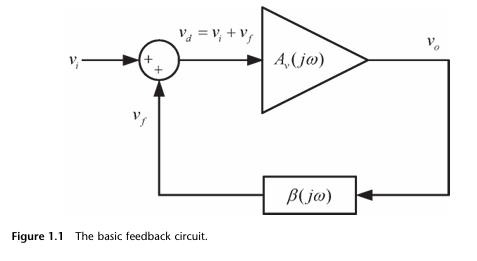
\includegraphics[width=0.6\linewidth]{images/oscilador-amplificador-feedback.png}
    \caption{Sistema de Feedback e Amplificação. \cite{gonzales2007}}
    \label{fig:oscilador-amplificador-feedback}
\end{figure}

No Logisim, esse circuito de oscilador será representado por este componente, nativo do simulador e com clock personável no próximo sistema.

\begin{figure}[H]
    \centering
    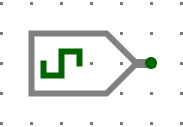
\includegraphics[width=0.2\linewidth]{images/clock-logisim.png}
    \caption{Clock no Logisim Evolution}
    \label{fig:clock-logisim}
\end{figure}